\chapter{Technical background}
This chapter presents an overview of the technical concepts involved in the realization of this project, namely the Ethereum Blockchain and Web applications
\section{Ethereum Blockchain}
Ethereum is a blockchain platform with its own \gls{cryptocurrency}, called Ether (ETH) or Ethereum, and its own programming language, called Solidity. As a blockchain network, Ethereum is a decentralized public ledger for verifying and recording transactions. The network's users can create, publish, monetize, and use applications on the platform, and use its Ether cryptocurrency as payment. Insiders call the decentralized applications on the network "dapps."\cite{ethereumcommunityEthereumDevelopmentDocumentation}.

\begin{wrapfigure}[10]{r}{4cm}
	\vspace{-10pt}
	
\includegraphics[width=4cm]{images/chapter2/ethereum.png}
	\vspace{-10pt}
	\caption{{\footnotesize Ethereum Blockchain logo}}
\end{wrapfigure}

Ethereum intends to create an alternative protocol for building decentralized applications, providing a different set of tradeoffs that its creators believe will be very useful for a large class of decentralized applications, with particular emphasis on situations where rapid development time, security for small and rarely used applications, and the ability of different applications to very efficiently interact, are important. Ethereum does this by building what is essentially the ultimate abstract foundational layer: a blockchain with a built-in Turing-complete programming language, allowing anyone to write smart contracts and decentralized applications where they can create their own arbitrary rules for ownership, transaction formats and state transition functions.

In the Ethereum universe, there is a single, canonical computer (called the Ethereum Virtual Machine, or EVM) whose state everyone on the Ethereum network agrees on. Everyone who participates in the Ethereum network (every Ethereum node) keeps a copy of the state of this computer. Additionally, any participant can broadcast a request for this computer to perform arbitrary computation. Whenever such a request is broadcast, other participants on the network verify, validate, and carry out ("execute") the computation. This causes a state change in the EVM, which is committed and propagated throughout the entire network.

\subsection{Accounts}
In Ethereum, the state is made up of objects called "accounts", with each account having a 20-byte address and state transitions being direct transfers of value and information between accounts. An Ethereum account contains four fields:

\begin{itemize}
\item The \textbf{nonce}, a counter used to make sure each transaction can only be processed once
\item The account's current \textbf{ether} balance
\item The account's \textbf{contract code}, if present
\item The account's \textbf{storage} (empty by default)
\end{itemize}

"Ether" is the main internal crypto-fuel of Ethereum, and is used to pay transaction fees. In general, there are two types of accounts: \textbf{externally owned accounts}, controlled by private keys, and \textbf{contract accounts}, controlled by their contract code. An externally owned account has no code, and one can send messages from an externally owned account by creating and signing a transaction; in a contract account, every time the contract account receives a message its code activates, allowing it to read and write to internal storage and send other messages or create contracts in turn.\newpage

\begin{figure}[h]
	\centering
		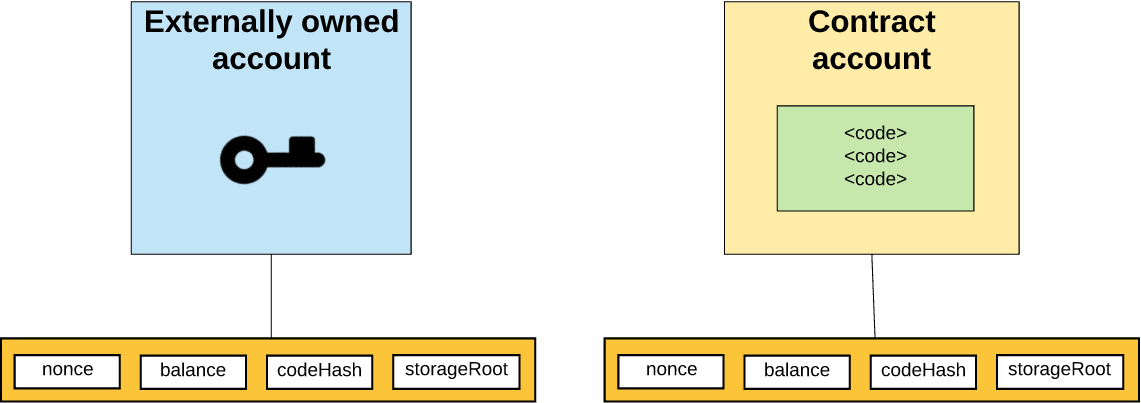
\includegraphics[width=10cm]{images/chapter2/accounts.png}
		\caption{{\footnotesize Abstract Ethereum accounts visualization}}
\end{figure}

\subsection{Transactions}
An Ethereum transaction refers to an action initiated by an externally-owned account, in other words an account managed by a human, not a contract. For example, if Bob sends Alice 1 ETH, Bob's account must be debited and Alice's must be credited. This state-changing action takes place within a transaction.

\begin{figure}[H]
	\centering
		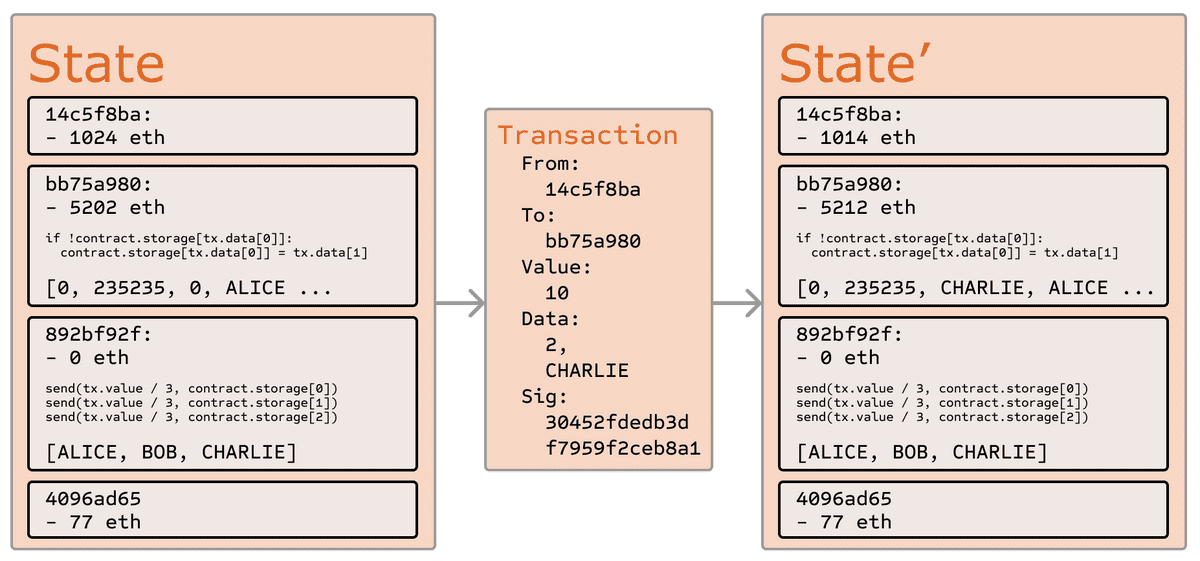
\includegraphics[width=10cm]{images/chapter2/transition.png}
		\caption{{\footnotesize Abstract representation of an Ethereum transaction}}
\end{figure}

Transactions, which change the state of the EVM, need to be broadcast to the whole network. Any node can broadcast a request for a transaction to be executed on the EVM; after this happens, a miner will execute the transaction and propagate the resulting state change to the rest of the network.

Transactions require a fee and must be mined to become valid.

A submitted transaction includes the following information:

\begin{itemize}
\item \textbf{recipient} - the receiving address (if an externally-owned account, the transaction will transfer value. If a contract account, the transaction will execute the contract code)
\item \textbf{signature} - the identifier of the sender. This is generated when the sender's private key signs the transaction and confirms the sender has authorised this transaction
\item \textbf{value} - amount of ETH to transfer from sender to recipient (in WEI, a denomination of ETH)
\item \textbf{data} - optional field to include arbitrary data
\item \textbf{gasLimit} - the maximum amount of gas units that can be consumed by the transaction. Units of gas represent computational steps
\item \textbf{gasPrice} - the fee the sender pays per unit of gas
\end{itemize}

Gas is a reference to the computation required to process the transaction by a miner. Users have to pay a fee for this computation. The gasLimit and gasPrice determine the maximum transaction fee paid to the miner (more on gas on later subsections.

\subsection{Gas}
Gas refers to the unit that measures the amount of computational effort required to execute specific operations on the Ethereum network.

Since each Ethereum transaction requires computational resources to execute, each transaction requires a fee. Gas refers to the fee required to successfully conduct a transaction on Ethereum.

\begin{figure}[h]
	\centering
		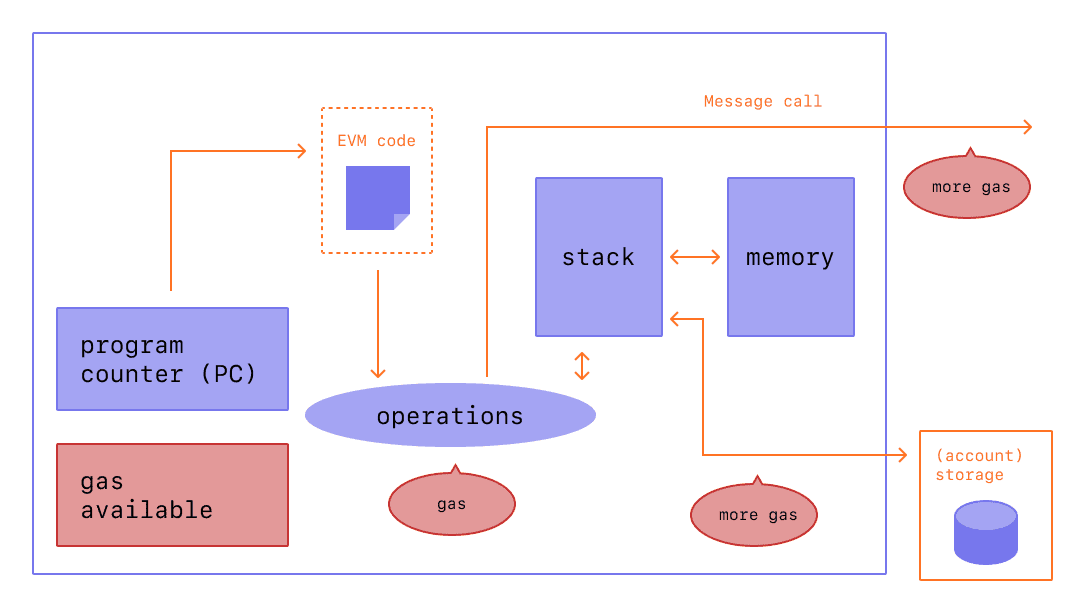
\includegraphics[width=10cm]{images/chapter2/gas.png}
		\caption{{\footnotesize Diagram of the role of gas in Ethereum \cite{taniTakenobuhsEthereumevmillustratedOnline2021}}}
\end{figure}

In essence, gas fees are paid in Ethereum's native currency, ether (ETH). Gas prices are denoted in gwei, which itself is a denomination of ETH - each gwei is equal to 0.000000001 ETH (10-9 ETH). For example, instead of saying that your gas costs 0.000000001 ether, you can say your gas costs 1 gwei.

Gas fees exist because they help keep the Ethereum network secure. By requiring a fee for every computation executed on the network, we prevent actors from spamming the network. In order to prevent accidental or hostile infinite loops or other computational wastage in code, each transaction is required to set a limit to how many computational steps of code execution it can use. The fundamental unit of computation is "gas".

\subsection{Consensus mechanisms}
When it comes to blockchains like Ethereum, which are in essence distributed databases, the nodes of the network must be able to reach agreement on the current state of the system. This is achieved using consensus mechanisms.

Consensus mechanisms (also known as consensus protocols or consensus algorithms) allow distributed systems (networks of computers) to work together and stay secure.

For decades, these mechanisms have been used to establish consensus among database nodes, application servers, and other enterprise infrastructure. In recent years, new consensus protocols have been invented to allow \gls{cryptoeconomic} systems, such as Ethereum, to agree on the state of the network.

A consensus mechanism in a cryptoeconomic system also helps prevent certain kinds of economic attacks. In theory, an attacker can compromise consensus by controlling 51\% of the network. Consensus mechanisms are designed to make this "\gls{51attack}" unfeasible. Different mechanisms are engineered to solve this security problem differently.
\subsubsection{Types of consensus mechanisms}

\begin{description}
\item[Proof of work] Proof-of-work is done by miners, who compete to create new blocks full of processed transactions. The winner shares the new block with the rest of the network and earns some freshly minted \gls{ETH}. The race is won by whoever's computer can solve a math puzzle fastest – this produces the cryptographic link between the current block and the block that went before. Solving this puzzle is the work in "proof of work".
\item[Proof of stake] Proof-of-stake is done by validators who have staked ETH to participate in the system. A validator is chosen at random to create new blocks, share them with the network and earn rewards. Instead of needing to do intense computational work, you simply need to have staked your ETH in the network. This is what incentivises healthy network behaviour.
\end{description}

\subsection{Dapps}

A dapp has its backend code running on a decentralized peer-to-peer network. Contrast this with an app where the backend code is running on centralized servers.

A dapp can have frontend code and user interfaces written in any language (just like an app) that can make calls to its backend. Furthermore, its frontend can be hosted on decentralized storage.

\begin{description}
\item[Decentralized] means they are independent, and no one can control them as a group.
\item[Deterministic] they perform the same function irrespective of the environment they are executed.
\item[Turing complete] which means given the required resources, the dapp can perform any action.
\item[Isolated] which means they are executed in a virtual environment known as Ethereum Virtual Machine so that if the smart contract happens to have a bug, it won’t hamper the normal functioning of the blockchain network.
\end{description}

\begin{figure}[H]
	\centering
		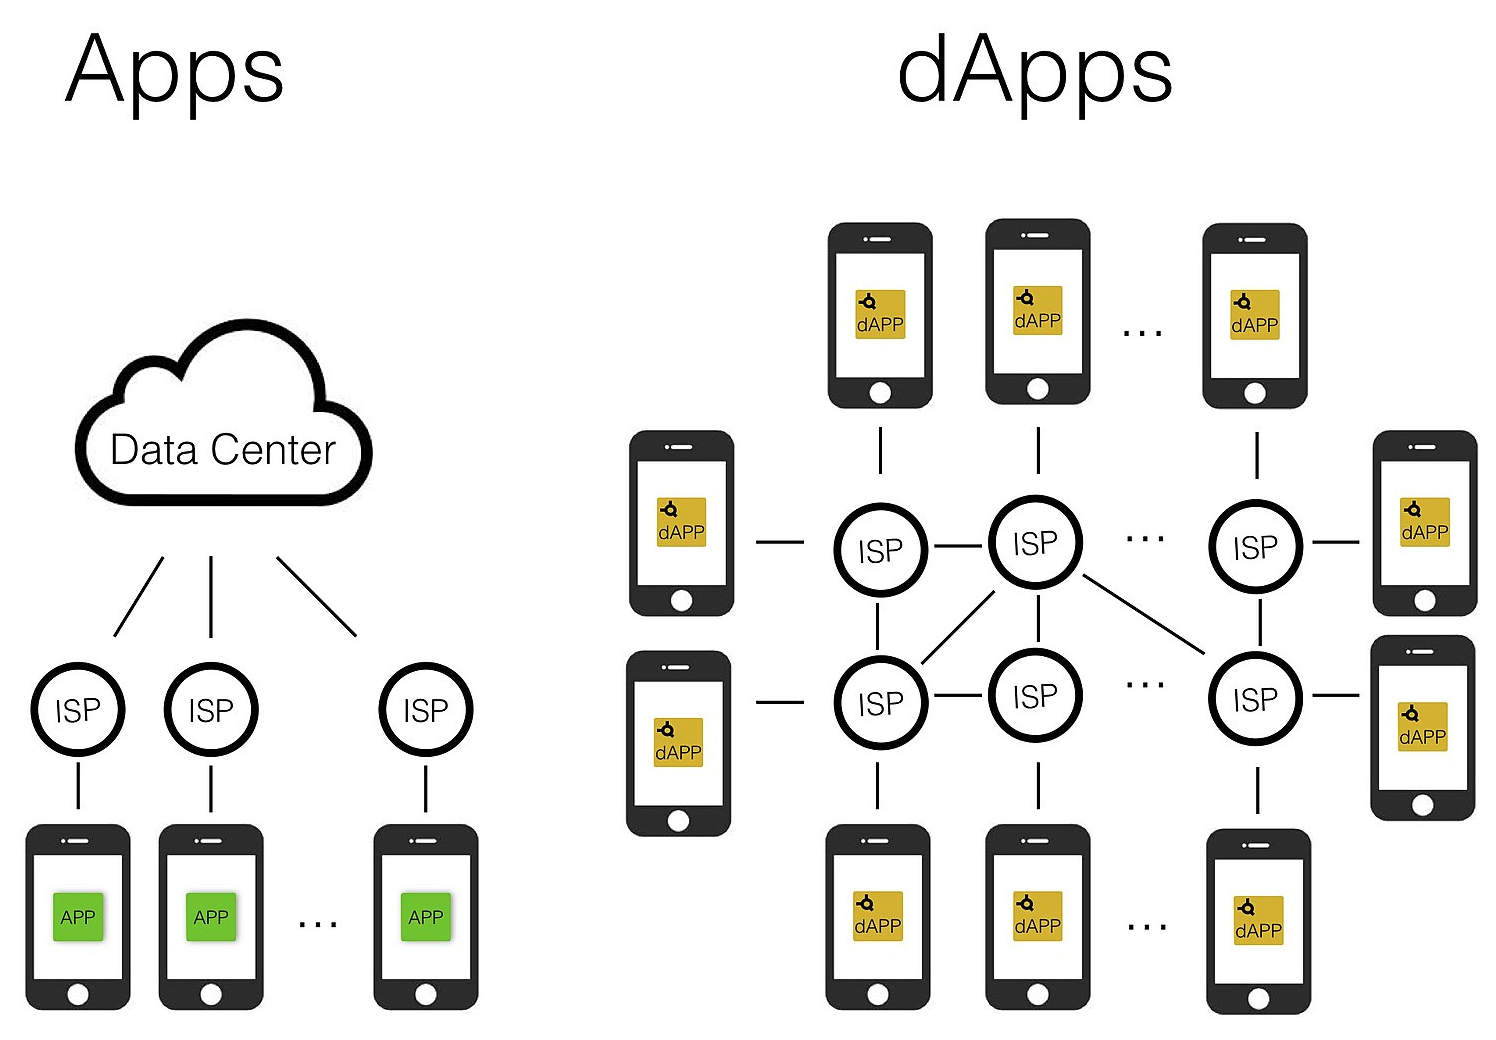
\includegraphics[width=10cm]{images/chapter2/dapps.png}
		\caption{{\footnotesize Diagram of centralized and decentralized applications topology}}
\end{figure}

\subsection{Smart contracts}

A smart contract is simply put a program that runs on the Ethereum blockchain. It's a collection of code (its functions) and data (its state) that resides at a specific address on the Ethereum blockchain. They run exactly as programmed. Once they are deployed on the network they can't be changed. Dapps can be decentralized because they are controlled by the logic written into the contract, not an individual or company.

Smart contracts are a type of Ethereum account. This means they have a balance and they can send transactions over the network. User accounts can then interact with a smart contract by submitting transactions that execute a function defined on the smart contract. Smart contracts can define rules, like a regular contract, and automatically enforce them via the code.\medskip

Ethereum has developer-friendly languages for writing smart contracts:

\begin{itemize}
\item Solidity
\item Vyper 
\end{itemize}

\section{Web Applications}

A web application (or web app) is application software that runs on a web server, unlike computer-based software programs that are run locally on the operating system (OS) of the device. Web applications are accessed by the user through a web browser with an active network connection. These applications are programmed using a client–server modeled structure—the user ("client") is provided services through an off-site server that is hosted by a third-party. Examples of commonly-used web applications include: web-mail, online retail sales, online banking, and online auctions.

\subsection{Structure}

Applications are usually broken into logical chunks called "tiers", where every tier is assigned a role. Traditional applications consist only of 1 tier, which resides on the client machine, but web applications lend themselves to an n-tiered approach by nature. Though many variations are possible, the most common structure is the three-tiered application.\cite{krunalMakeNtierArchitecture2008} In its most common form, the three tiers are called presentation, application and storage, in this order. A web browser is the first tier (presentation), an engine using some dynamic Web content technology (such as ASP, CGI, ColdFusion, Dart, JSP/Java, Node.js, PHP, Python or Ruby on Rails) is the middle tier (application logic), and a database is the third tier (storage). The web browser sends requests to the middle tier, which services them by making queries and updates against the database and generates a user interface.

For more complex applications, a 3-tier solution may fall short, and it may be beneficial to use an n-tiered approach, where the greatest benefit is breaking the business logic, which resides on the application tier, into a more fine-grained model.\cite{krunalMakeNtierArchitecture2008} Another benefit may be adding an integration tier that separates the data tier from the rest of tiers by providing an easy-to-use interface to access the data. For example, the client data would be accessed by calling a "list\_clients()" function instead of making an SQL query directly against the client table on the database. This allows the underlying database to be replaced without making any change to the other tiers.

There are some who view a web application as a two-tier architecture. This can be a "smart" client that performs all the work and queries a "dumb" server, or a "dumb" client that relies on a "smart" server. The client would handle the presentation tier, the server would have the database (storage tier), and the business logic (application tier) would be on one of them or on both.\cite{krunalMakeNtierArchitecture2008} While this increases the scalability of the applications and separates the display and the database, it still doesn't allow for true specialization of layers, so most applications will outgrow this model.

\subsection{Business use}

An emerging strategy for application software companies is to provide web access to software previously distributed as local applications. Depending on the type of application, it may require the development of an entirely different browser-based interface, or merely adapting an existing application to use different presentation technology. These programs allow the user to pay a monthly or yearly fee for use of a software application without having to install it on a local hard drive. A company which follows this strategy is known as an application service provider (ASP), and ASPs are currently receiving much attention in the software industry.

Security breaches on these kinds of applications are a major concern because it can involve both enterprise information and private customer data. Protecting these assets is an important part of any web application and there are some key operational areas that must be included in the development process. This includes processes for authentication, authorization, asset handling, input, and logging and auditing. Building security into the applications from the beginning can be more effective and less disruptive in the long run.

Cloud computing model web applications are software as a service (SaaS). There are business applications provided as SaaS for enterprises for a fixed or usage-dependent fee. Other web applications are offered free of charge, often generating income from advertisements shown in web application interface\cite{curtisfranklinjrTopTipsSecure2011}.

\subsection{Development}

Writing web applications is often simplified by the use of web application framework. These frameworks facilitate rapid application development by allowing a development team to focus on the parts of their application which are unique to their goals without having to resolve common development issues such as user management. Many of the frameworks in use are open-source software.

The use of web application frameworks can often reduce the number of errors in a program, both by making the code simpler, and by allowing one team to concentrate on the framework while another focuses on a specified use case. In applications which are exposed to constant hacking attempts on the Internet, security-related problems can be caused by errors in the program. Frameworks can also promote the use of best practices such as GET after POST.

In addition, there is potential for the development of applications on Internet operating systems, although currently there are not many viable platforms that fit this model\cite{docforgeFrameworkDocForgeProgramming2010}.